% Compile with XeLaTeX or LuaLaTeX.
\documentclass[aspectratio=169,11pt]{beamer}

\usepackage{fontspec}
\usepackage{microtype}
\usepackage{mathtools}
\usepackage{unicode-math}
\usepackage{booktabs}
\usepackage{tabularx}
\usepackage{array}
\usepackage{tikz}
\usepackage{colortbl}
\usepackage{ragged2e}
\usepackage{enumitem}
\usepackage{mathtools}
\usepackage{graphicx}
\usepackage{adjustbox}
\usepackage{multirow}

\usetikzlibrary{arrows.meta,positioning,calc,fit,backgrounds}

% --- Fonts: clean, modern, widely available in TeX Live ---
\setmainfont{Nimbus Sans}
\setsansfont{Nimbus Sans}
\setmonofont{DejaVu Sans Mono}
\setmathfont{DejaVu Math TeX Gyre}

% --- Beamer theme ---
\usefonttheme{professionalfonts}
\usetheme[numbering=fraction,progressbar=frametitle]{metropolis}
% \usetheme[numbering=fraction,progressbar=frametitle]{metropolis}
\metroset{block=fill}
\setbeamertemplate{navigation symbols}{}
\setbeamertemplate{caption}{\raggedright\insertcaption\par}
\setbeamertemplate{itemize items}[circle]
\setbeamertemplate{enumerate items}[default]

% --- Colors ---
\definecolor{Navy}{HTML}{0B1F3A}
\definecolor{Teal}{HTML}{0F766E}
\definecolor{Slate}{HTML}{475569}
\definecolor{SoftBg}{HTML}{F8FAFC}
\definecolor{Accent}{HTML}{2563EB}
\definecolor{WarmGray}{HTML}{64748B}
\definecolor{SITRed}{HTML}{C41230}

\setbeamercolor{normal text}{fg=Slate,bg=white}
\setbeamercolor{alerted text}{fg=Teal}
\setbeamercolor{frametitle}{fg=Navy,bg=white}
\setbeamercolor{progress bar}{fg=Teal,bg=SoftBg}
\setbeamercolor{block title}{fg=white,bg=Navy}
\setbeamercolor{block body}{fg=Slate,bg=SoftBg}
\setbeamercolor{block title alerted}{fg=white,bg=Teal}
\setbeamercolor{block body alerted}{fg=Slate,bg=SoftBg}
\setbeamercolor{block title example}{fg=white,bg=Accent}
\setbeamercolor{block body example}{fg=Slate,bg=SoftBg}
\setbeamercolor{title}{fg=Navy}
\setbeamercolor{subtitle}{fg=Slate}
\setbeamercolor{section in toc}{fg=Navy}
\setbeamercolor{structure}{fg=Teal}

% --- Typography / spacing ---
\setlist[itemize]{leftmargin=1.2em,itemsep=0.35em,topsep=0.35em}
\setlist[enumerate]{leftmargin=1.3em,itemsep=0.35em,topsep=0.35em}
\setlength{\parskip}{0.4em}
\setlength{\parindent}{0pt}
\RaggedRight

\newcommand{\kw}[1]{\textbf{#1}}
\newcommand{\mono}[1]{\texttt{#1}}
\newcommand{\smalltag}[1]{\textcolor{WarmGray}{\footnotesize #1}}

\title{A Generalisable Pipeline for Backporting ROCm to Obsolete AMD Hardware}
\subtitle{Executive summary deck for technical mentorship}
\author{Soham Kulkarni}
\date{}

\begin{document}

% --- Slide 1 ---
\begin{frame}[plain]
    \vspace{0.8cm}
    {\LARGE\bfseries\color{Navy} A Generalisable Pipeline for Backporting ROCm to Obsolete AMD Hardware}\par
    \vspace{0.25cm}
    {\large\color{Slate} Executive summary for technical mentorship}\par
    \vspace{0.9cm}

    \begin{block}{Core thesis}
        \large
        Build a \kw{reusable, benchmarked recovery pipeline} for dropped AMD GPU support in ROCm, so older hardware can be revived without rediscovering the same failure modes from scratch.
    \end{block}

    \vfill
    \smalltag{Source-constrained summary based on the provided project draft; no funding language included.}
\end{frame}

% --- Slide 2 ---
\begin{frame}{Why this matters}
    \begin{columns}[T,onlytextwidth]
        \column{0.58\textwidth}
        \begin{block}{Problem in one sentence}
            ROCm is the only credible open-source alternative to CUDA for GPU compute, but AMD periodically drops support for older architectures.
        \end{block}

        \begin{itemize}
            \item Capable hardware becomes \kw{software-stranded} rather than physically obsolete.
            \item This is especially acute for cost-constrained users relying on Ryzen APUs and Vega-class GPUs.
            \item The gap is not a hardware failure; it is a missing migration path.
        \end{itemize}

        \column{0.42\textwidth}
        \begin{block}{What the project targets}
            \begin{itemize}
                \item dropped GPU support
                \item fragmented community fixes
                \item missing reproduction steps
                \item unclear performance cost
            \end{itemize}
        \end{block}
    \end{columns}
\end{frame}

% --- Slide 3 ---
\begin{frame}{The gap: support exists in fragments, not as a workflow}
    \begin{columns}[T,onlytextwidth]
        \column{0.48\textwidth}
        \begin{block}{Current reality}
            \begin{itemize}
                \item scattered forum posts and issue threads
                \item ad hoc workarounds
                \item no single end-to-end reference
                \item little evidence about trade-offs
            \end{itemize}
        \end{block}

        \column{0.48\textwidth}
        \begin{block}{What is missing}
            \begin{itemize}
                \item reproducible steps
                \item benchmarked comparisons
                \item clear failure boundaries
                \item a path others can reuse
            \end{itemize}
        \end{block}
    \end{columns}

    \vspace{0.2cm}
    \begin{alertblock}{Research gap}
        Existing recovery attempts are \kw{not systematised, not benchmarked, and not reproducible}.
    \end{alertblock}
\end{frame}

% --- Slide 4 ---
\begin{frame}{Proposed approach: a decision tree for recovery}
    \centering
    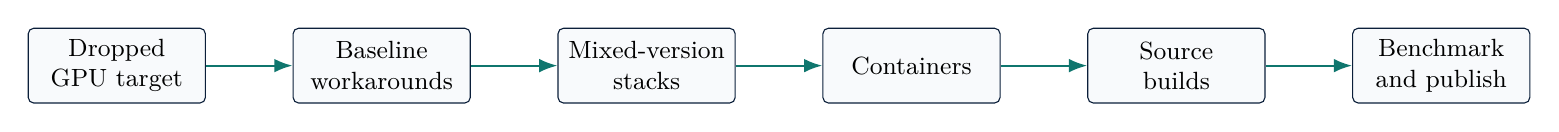
\begin{tikzpicture}[
        node distance=1.2cm and 1.1cm,
        every node/.style={font=\small},
        box/.style={draw=Navy, rounded corners=2pt, align=center, minimum height=0.95cm, minimum width=2.25cm, fill=SoftBg},
        arrow/.style={-Latex, thick, draw=Teal}
    ]
        \node[box] (a) {Dropped\\GPU target};
        \node[box, right=of a] (b) {Baseline\\workarounds};
        \node[box, right=of b] (c) {Mixed-version\\stacks};
        \node[box, right=of c] (d) {Containers};
        \node[box, right=of d] (e) {Source\\builds};
        \node[box, right=of e] (f) {Benchmark\\and publish};

        \draw[arrow] (a) -- (b);
        \draw[arrow] (b) -- (c);
        \draw[arrow] (c) -- (d);
        \draw[arrow] (d) -- (e);
        \draw[arrow] (e) -- (f);
    \end{tikzpicture}

    \vspace{0.45cm}
    \begin{block}{Key idea}
        The project is a \kw{systematic pipeline}, not a one-off workaround: each strategy isolates a different failure layer and each successful configuration is measured.
    \end{block}
\end{frame}

% --- Slide 5 ---
\begin{frame}{Recovery strategies under test}
    \small
    \begin{tabularx}{\textwidth}{>{\bfseries}p{3.1cm}X p{4.1cm}}
        \toprule
        Strategy & Idea & What it tells us \\
        \midrule
        Community baseline & Environment-level spoofing and existing workarounds & How far unsupported hardware runs without rebuilding the stack \\
        Mixed-version stacks & ROCm userspace and AMDGPU kernel version decoupling & Whether failures come from driver ABI, userspace, or missing architecture support \\
        Containerised vendor stacks & AMD Docker images across ROCm versions & Whether containers preserve the last usable stack or recover lost support \\
        Source builds & Rebuild PyTorch and ROCm components with explicit targets & Whether compilation alone restores missing functionality \\
        \bottomrule
    \end{tabularx}

    \vspace{0.35cm}
    \begin{alertblock}{Design principle}
        Start with the least invasive path, then move toward more expensive interventions only when they add diagnostic value.
    \end{alertblock}
\end{frame}

% --- Slide 6 ---
\begin{frame}[shrink=8]{Scope: two representative targets, one reusable method}
    \begin{columns}[T,onlytextwidth]
        \column{0.50\textwidth}
        \begin{block}{Initial hardware targets}
            \begin{itemize}
                \item \mono{gfx90c} — Ryzen 5 5650U / Cezanne APU / Vega 7
                \item \mono{gfx902} — Ryzen 5 2200G / Raven Ridge / Vega 8
            \end{itemize}
        \end{block}

        \begin{block}{Why these two}
            \begin{itemize}
                \item laptop and desktop form factors
                \item same architectural family, different systems
                \item useful cross-check for generalisation
            \end{itemize}
        \end{block}

        \column{0.50\textwidth}
        \begin{block}{Reference environments from the draft}
            \begin{itemize}
                \item Fedora 43 on the 5650U system
                \item RHEL 9.5 on the 2200G desktop
                \item system ROCm 6.4.4 on the current host setup
            \end{itemize}
        \end{block}

        \begin{block}{Generalisation goal}
            The first traversal is about these two targets; the methodology is intended to transfer to other dropped AMD architectures later.
        \end{block}
    \end{columns}
\end{frame}

% --- Slide 7 ---
\begin{frame}[shrink=8]{How success will be measured}
    \begin{columns}[T,onlytextwidth]
        \column{0.56\textwidth}
        \begin{block}{Evaluation at every stage}
            \begin{itemize}
                \item direct HIP execution
                \item PyTorch runtime behavior
                \item performance relative to a working baseline
                \item reproducibility across systems and versions
            \end{itemize}
        \end{block}

        \begin{block}{Comparison anchors in the draft}
            \begin{itemize}
                \item latest stable ROCm for the target
                \item AMD's published theoretical figures
                \item observed results from the current workaround path
            \end{itemize}
        \end{block}

        \column{0.44\textwidth}
        \begin{exampleblock}{Initial observation from the draft}
            The current \mono{gfx900} spoof path for \mono{gfx90c} reportedly reaches about \kw{50\%} of AMD's published figures for the Vega 7.
        \end{exampleblock}

        \smalltag{This is retained because it appears explicitly in the source draft and motivates the benchmarking plan.}
    \end{columns}
\end{frame}

% --- Slide 8 ---
\begin{frame}[shrink=8]{What has already been established}
    \begin{columns}[T,onlytextwidth]
        \column{0.50\textwidth}
        \begin{block}{Post 1: context and motivation}
            Frames the ROCm ecosystem, the hardware target, and the case for running modern ML tooling on dropped \mono{GCN5} hardware.
        \end{block}

        \column{0.50\textwidth}
        \begin{block}{Post 2: installation and problem identification}
            Shows native \mono{ROCm 6.4.4} installation via Fedora's DNF metapackage, successful HIP execution, and the central blocker: missing \mono{gfx90c} kernels in bundled rocBLAS for PyTorch.
        \end{block}
    \end{columns}

    \vspace{0.35cm}
    \begin{alertblock}{Status signal}
        The hardware compute stack is functional; the unresolved issue is support continuity in ROCm userspace and packaged kernels.
    \end{alertblock}
\end{frame}

% --- Slide 9 ---
\begin{frame}[shrink=8]{Execution path: from diagnosis to validation}
    \begin{columns}[T,onlytextwidth]
        \column{0.33\textwidth}
        \begin{block}{1. Baseline}
            Test existing workarounds and identify the first failure layer.
        \end{block}

        \begin{block}{2. Decouple}
            Mix ROCm userspace and AMDGPU versions to isolate compatibility boundaries.
        \end{block}

        \column{0.33\textwidth}
        \begin{block}{3. Containerise}
            Compare AMD Docker images across ROCm versions on the same host stack.
        \end{block}

        \begin{block}{4. Rebuild}
            Compile PyTorch and, where needed, ROCm components with explicit architecture targeting.
        \end{block}

        \column{0.33\textwidth}
        \begin{block}{5. Validate}
            Re-run successful configurations on \mono{gfx902} to test generalisation.
        \end{block}

        \begin{block}{6. Document}
            Publish the reproduction steps, benchmarks, and failure modes openly.
        \end{block}
    \end{columns}
\end{frame}

% --- Slide 10 ---
\begin{frame}[shrink=8]{Why mentorship would matter}
    \begin{columns}[T,onlytextwidth]
        \column{0.58\textwidth}
        \begin{block}{What I am trying to validate}
            Whether dropped AMD GPU support can be recovered through a reproducible sequence of spoofing, stack separation, containerisation, and selective source builds — with benchmarks at every stage.
        \end{block}

        \begin{itemize}
            \item tighten the technical methodology
            \item pressure-test the feasibility boundaries
            \item avoid dead ends that look promising but do not scale
            \item turn one hardware case into a reusable playbook
        \end{itemize}

        \column{0.42\textwidth}
        \begin{exampleblock}{Mentorship ask}
            Review the technical approach, benchmark discipline, and recovery strategy ordering so the work stays rigorous and generalisable.
        \end{exampleblock}

        \vspace{0.3cm}
        \begin{block}{Closing line}
            The objective is not just to make one GPU work; it is to build a method that others can apply when ROCm drops the next architecture.
        \end{block}
    \end{columns}
\end{frame}

\end{document}